\documentclass[border=10pt]{standalone}

\usepackage[utf8]{inputenc}
\usepackage[english]{babel}
\usepackage{tikz}
\usetikzlibrary{positioning, arrows.meta, fit}

\tikzset{
  neuron/.style={
    circle, draw, thick, 
    minimum size=1cm,
    node distance=0.05cm and 1cm
  },
  group/.style={ 
    rectangle,draw,thick, 
    inner sep=0pt, % no padding between the node contents and the rectangle shape
  },
  conn/.style={ % style for the connections
    -{Straight Barb[angle=60:2pt 3]}, % simple barbed arrow tip
    thick, % draw in a thick weight to match other drawing elements
  },
}


\begin{document}
	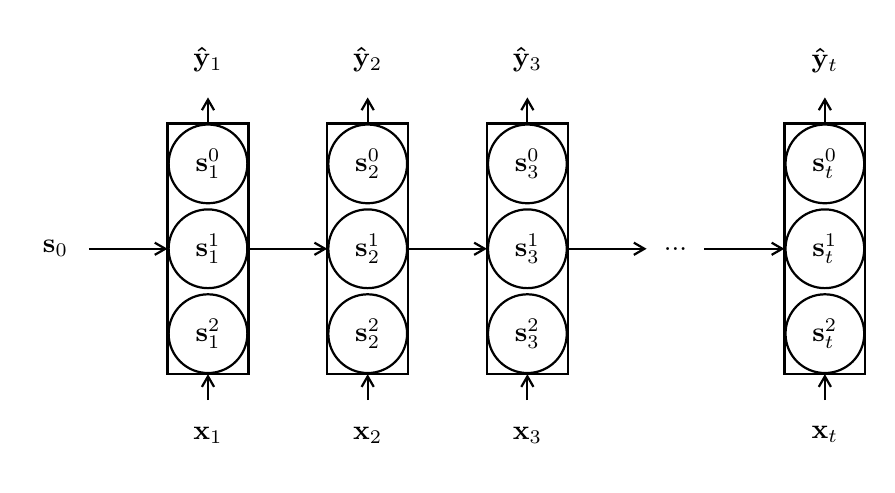
\begin{tikzpicture}
		% time step 0
		\node[neuron] (a00) {$\mathbf{s}_1^0$};
		\node[neuron,below=of a00] (a01) {$\mathbf{s}_1^1$};
		\node[neuron,below=of a01] (a02) {$\mathbf{s}_1^2$};
		\node[group,fit={(a00) (a01) (a02)}] (gr0) {};
		\node[outer sep=2, circle,above=0.33cm of a00] (y0) {$\mathbf{\hat{y}}_{1}$};
		\node[outer sep=2, circle,below=0.33cm of a02] (x0) {$\mathbf{x}_{1}$};
		\node[outer sep=2, circle,left=1cm of a01] (ainit) {$\mathbf{s}_{0}$};
		\draw[conn] (x0) -- (a02);
		\draw[conn] (a00) -- (y0);
		\draw[conn] (ainit) -- (a01);
		% time step 1
		\node[neuron, right=of a00] (a10) {$\mathbf{s}_2^0$};
		\node[neuron,below=of a10] (a11) {$\mathbf{s}_2^1$};
		\node[neuron,below=of a11] (a12) {$\mathbf{s}_2^2$};
		\node[group,fit={(a10) (a11) (a12)}] (gr1) {};
		\node[outer sep=2, circle, above=0.33cm of a10] (y1) {$\mathbf{\hat{y}}_{2}$};
		\node[outer sep=2, circle,below=0.33cm of a12] (x1) {$\mathbf{x}_{2}$};
		\draw[conn] (x1) -- (a12);
		\draw[conn] (a10) -- (y1);
		\draw[conn] (a01) -- (a11);
		% time step 2
		\node[neuron, right=of a10] (a20) {$\mathbf{s}_3^0$};
		\node[neuron,below=of a20] (a21) {$\mathbf{s}_3^1$};
		\node[neuron,below=of a21] (a22) {$\mathbf{s}_3^2$};
		\node[group,fit={(a20) (a21) (a22)}] (gr2) {};
		\node[outer sep=2, circle,above=0.33cm of a20] (y2) {$\mathbf{\hat{y}}_{3}$};
		\node[outer sep=2, circle,below=0.33cm of a22] (x2) {$\mathbf{x}_{3}$};
		\draw[conn] (x2) -- (a22);
		\draw[conn] (a20) -- (y2);
		\draw[conn] (a11) -- (a21);
		% ...
		\node[outer sep=2, circle] (punto) [right=of a21] {$...$};
		\draw[conn] (a21) -- (punto);
		% time step t
		\node[neuron, right= 2.75 cm of a20] (at0) {$\mathbf{s}_{t}^0$};
		\node[neuron,below=of at0] (at1) {$\mathbf{s}_{t}^1$};
		\node[neuron,below=of at1] (at2) {$\mathbf{s}_{t}^2$};
		\node[group,fit={(at0) (at1) (at2)}] (grt) {};
		\node[outer sep=2, circle,above=0.33cm of at0] (yt) {$\mathbf{\hat{y}}_{t}$};
		\node[outer sep=2, circle,below=0.33cm of at2] (xt) {$\mathbf{x}_{t}$};
		\draw[conn] (xt) -- (at2);
		\draw[conn] (at0) -- (yt);
		\draw[conn] (punto) -- (at1);
	\end{tikzpicture}
\end{document}